\section{Results}
    \subsection{Classification}
        % Table with the one best accuracy score from the two methods
        % Figure with analysis of regularization parameters and learning rates
        
%        Following are some results from the neural network classification project. Figure \ref{fig:ANNREG1} illustrates the accuracy scores for network $N3$:
%        \begin{figure}[H]
%            \centering
%            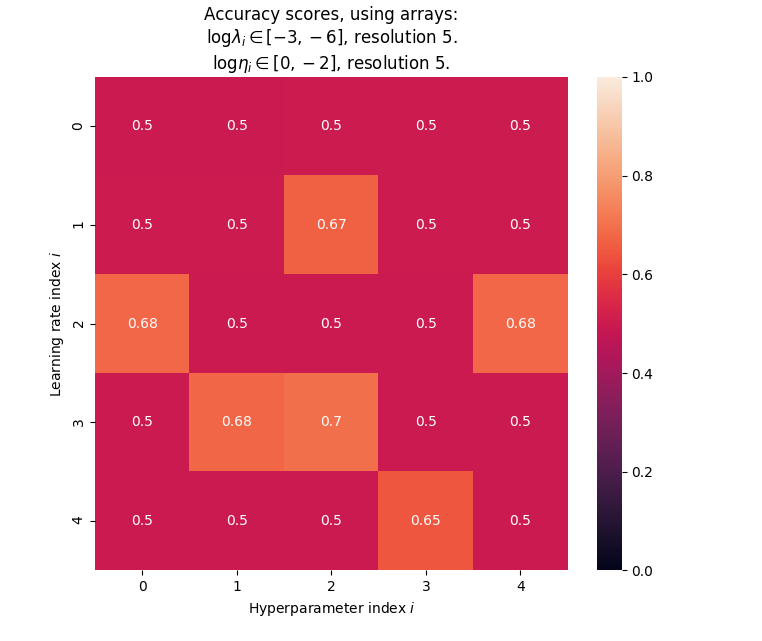
\includegraphics[width=0.4\textwidth]{figures/Ngrid3_acc.png}
%            \caption{Grid search with label $N3$ results. This figure illustrates the accuracy scores for several neural networks with various hyperparameters $\lambda$ and learning rates $\eta$. The range and resolutions of the parameters are in the title, while the indices of the axes range from largest to smallest.}
%            \label{fig:ANNREG1}
%        \end{figure}
%        Figure \ref{fig:ANNREG2} illustrates the area under the cumulative gain curve for network $N3$:
%        \begin{figure}[H]
%            \centering
%            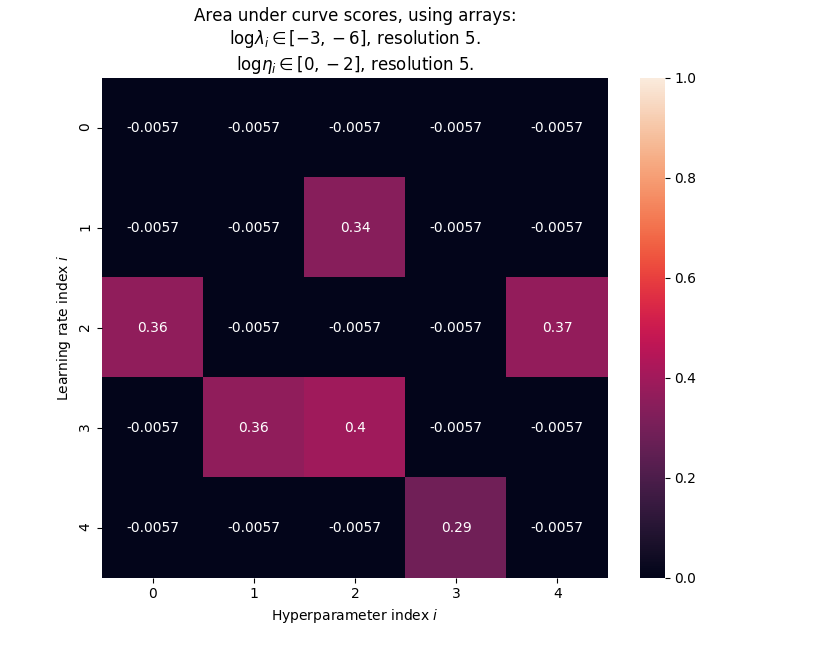
\includegraphics[width=0.4\textwidth]{figures/Ngrid3_auc.png}
%            \caption{Grid search with label $N3$ results. This figure illustrates the area under the cumulative gain curve for several neural networks with various hyperparameters $\lambda$ and learning rates $\eta$. The range and resolutions of the parameters are in the title, while the indices of the axes range from largest to smallest.}
%            \label{fig:ANNREG2}
%        \end{figure}
%        Figure \ref{fig:ANNREG3} illustrates the $F1$ scores for network $N3$:
%        \begin{figure}[H]
%            \centering
%            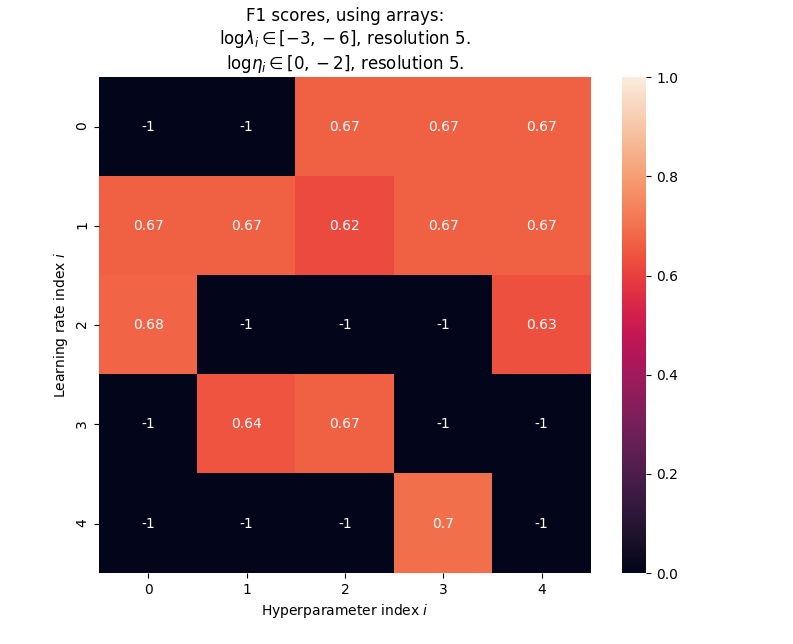
\includegraphics[width=0.4\textwidth]{figures/Ngrid3_F1.png}
%            \caption{Grid search with label $N3$ results. This figure illustrates the $F1$ for several neural networks with various hyperparameters $\lambda$ and learning rates $\eta$. The range and resolutions of the parameters are in the title, while the indices of the axes range from largest to smallest.}
%            \label{fig:ANNREG3}
%        \end{figure}

		The accurary score, F1-score, AUC-score and the gains-ratio of the classification neural network after studing the credit card data can be seen in figure \ref{fig:cc_acc}, \ref{fig:cc_F1}, \ref{fig:cc_auc} and \ref{fig:cc_gr} respectively.

		\begin{figure}[H]
			\centering
			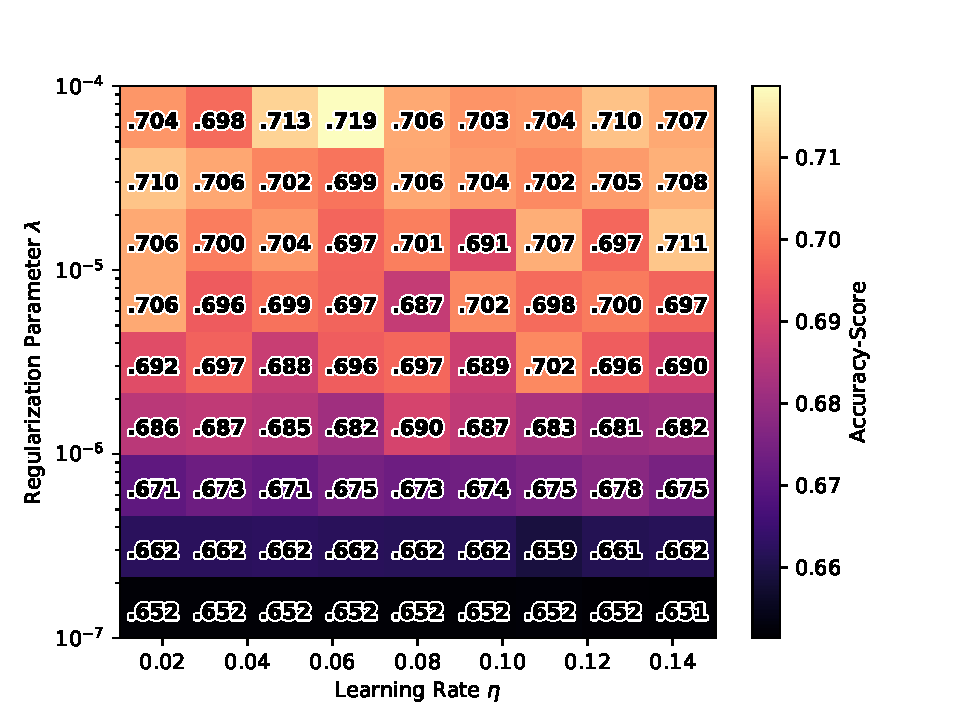
\includegraphics[width=0.5\textwidth]{figures/cc_res_0.pdf}
			\caption{The accurary score of the classification neural network for different $\eta$ and $\lambda$-values after studing the credit card data.}
			\label{fig:cc_acc}
		\end{figure}
		\begin{figure}[H]
			\centering
			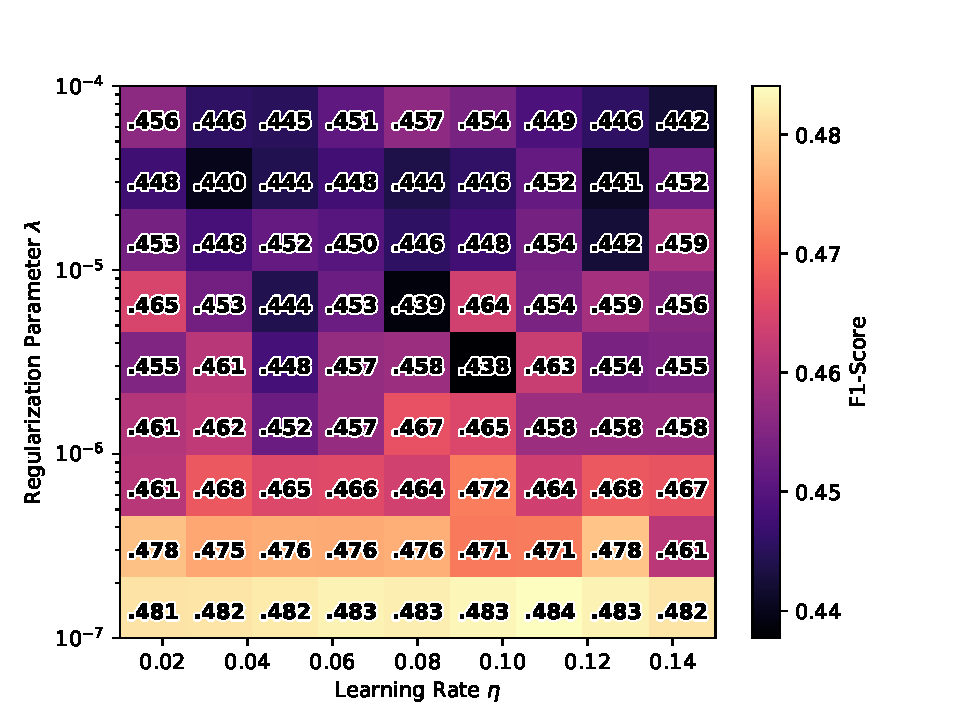
\includegraphics[width=0.5\textwidth]{figures/cc_res_1.pdf}
			\caption{The F1-score of the classification neural network for different $\eta$ and $\lambda$-values after studing the credit card data.}
			\label{fig:cc_F1}
		\end{figure}
		\begin{figure}[H]
			\centering
			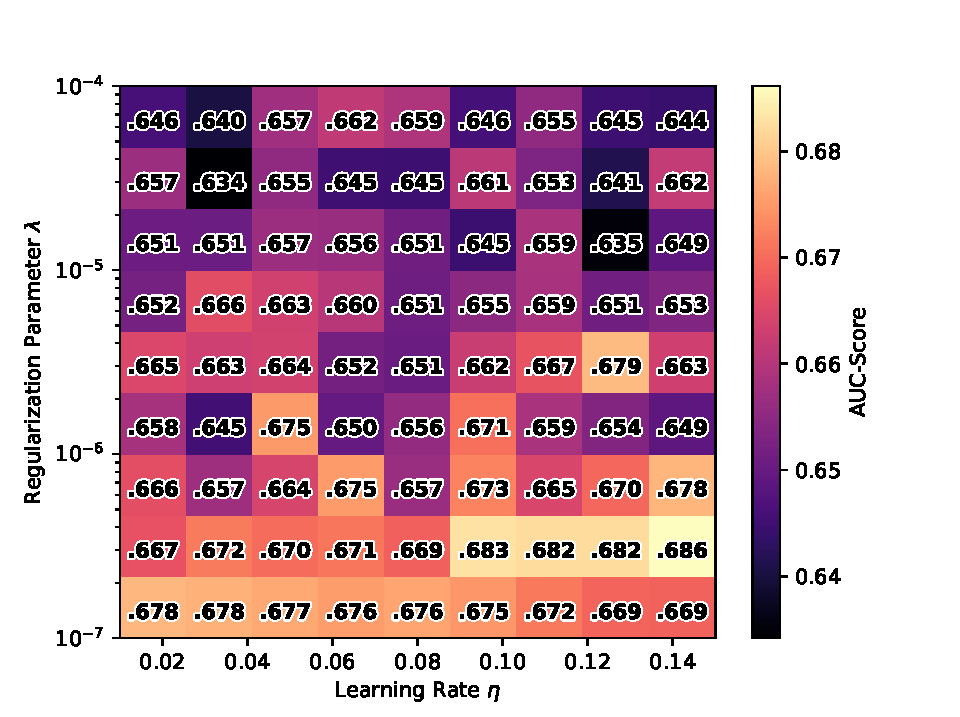
\includegraphics[width=0.5\textwidth]{figures/cc_res_2.pdf}
			\caption{The AUC-score of the classification neural network for different $\eta$ and $\lambda$-values after studing the credit card data.}
			\label{fig:cc_auc}
		\end{figure}
		\begin{figure}[H]
			\centering
			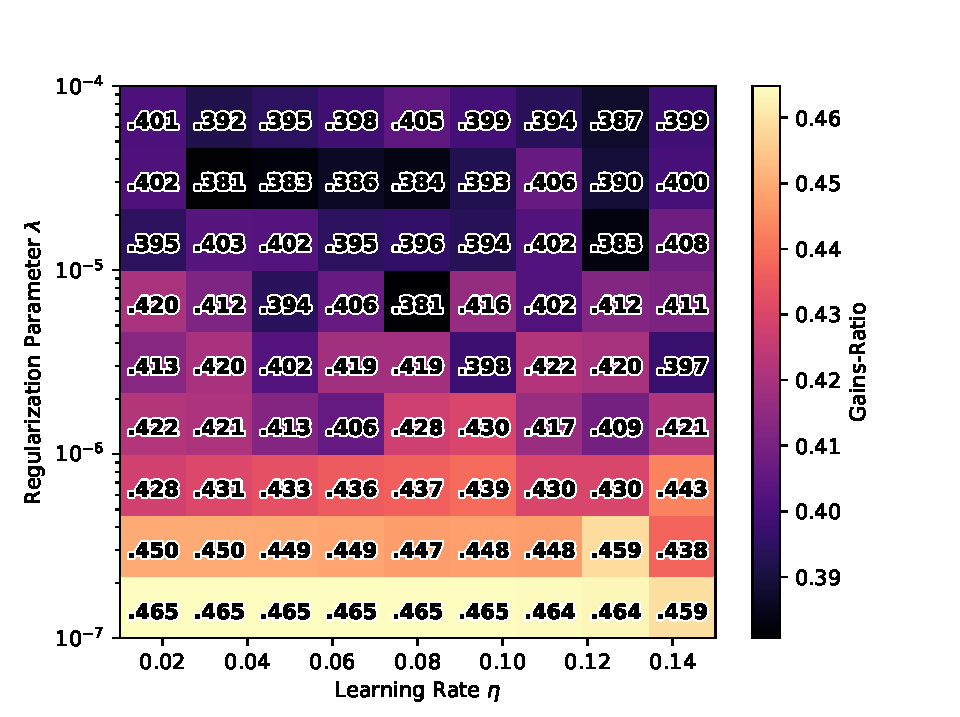
\includegraphics[width=0.5\textwidth]{figures/cc_res_3.pdf}
			\caption{The Gains-Ratio of the classification neural network for different $\eta$ and $\lambda$-values after studing the credit card data.}
			\label{fig:cc_gr}
		\end{figure}
	
        
        
    \subsection{Regression}
    
    	The mean squared error and the $R^2$-score of the regression neural network for different $\eta$ and $\lambda$-values after studing Franke's function can be seen in figure \ref{fig:ff_mse} and \ref{fig:ff_r2} respectively.
    
    	\begin{figure}[H]
    		\centering
    		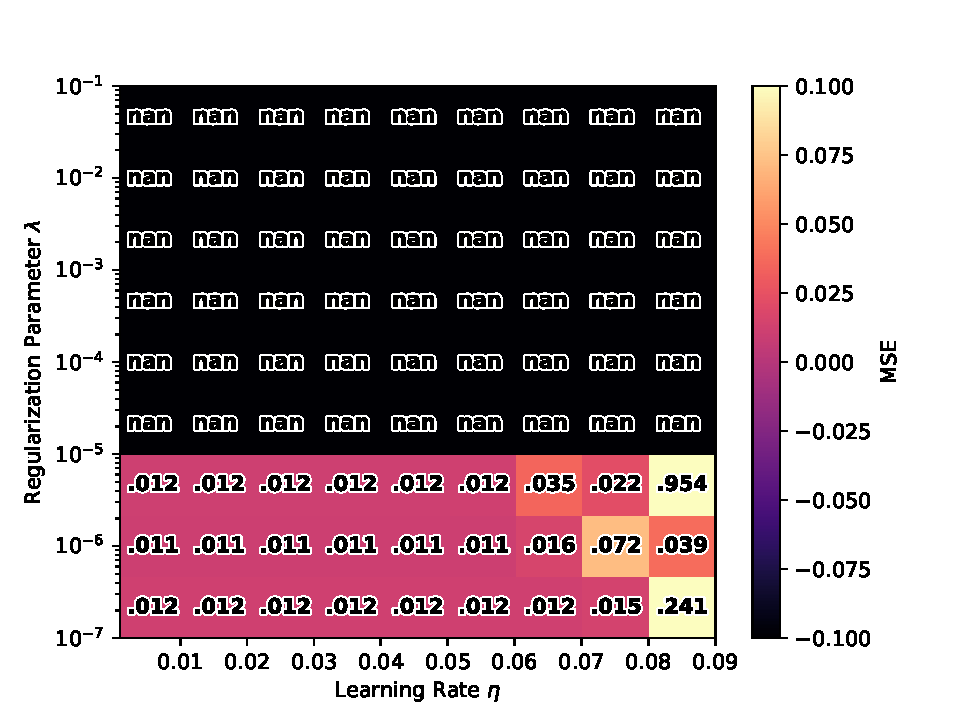
\includegraphics[width=0.5\textwidth]{figures/ff_res_0.pdf}
    		\caption{The mean squared error of the regression neural network for different $\eta$ and $\lambda$-values after studing Franke's function.}
    		\label{fig:ff_mse}
    	\end{figure}
    	\begin{figure}[H]
    		\centering
    		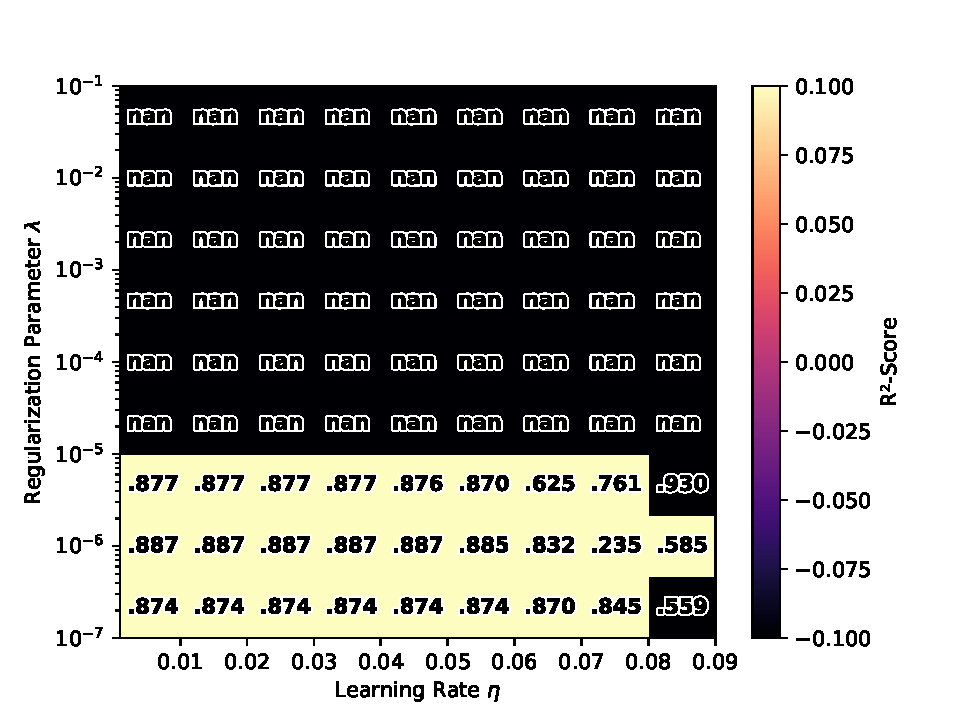
\includegraphics[width=0.5\textwidth]{figures/ff_res_1.pdf}
    		\caption{The $R^2$-score of the regression neural network after studing Franke's function.}
    		\label{fig:ff_r2}
    	\end{figure}
    
    
    	
%        Following is a table from project 1, listing the precision of three regression schemes applied to Franke's function:
%        \begin{table}[H]
%            \centering
%            \caption{Table listing the final results and comparisons of the regressional methods applied to Franke's function with $n=10,000$ data points.}
%            \begin{tabular}[t]{l@{\hskip 0.3in}c@{\hskip 0.3in}c@{\hskip 0.2in}c}
%                \toprule
%                Scheme & MSE minimum & $p_{deg}$ & $\log(\lambda)$ \\
%                \midrule
%                OLS & 0.2493 & 8 & $-$\\
%                Ridge & 0.2489 & 11 & -9\\
%                Lasso & 0.2524 & 8 & -12\\
%                \bottomrule
%            \end{tabular}
%            \label{tab:conclusion_table_Frankes}
%        \end{table}
%        
%        
%        \begin{figure}[H]
%            \centering
%            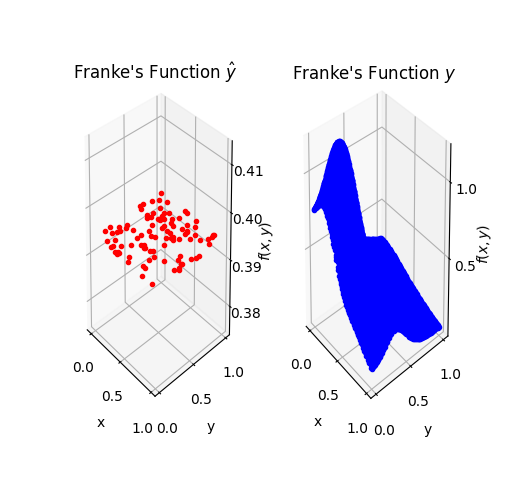
\includegraphics[width=0.4\textwidth]{figures/regression_NNW.png}
%            \caption{The ANN regression on Franke's function. With $MSE=4.08$.}
%            \label{fig:ANNREG}
%        \end{figure}
        
        
        % Table with the least MSE from the two methods
        % (Figure with analysis of regularization parameters and learning rates): this is not specifically asked for in the problem set, it wants: a discussion of reg. params./learning rates